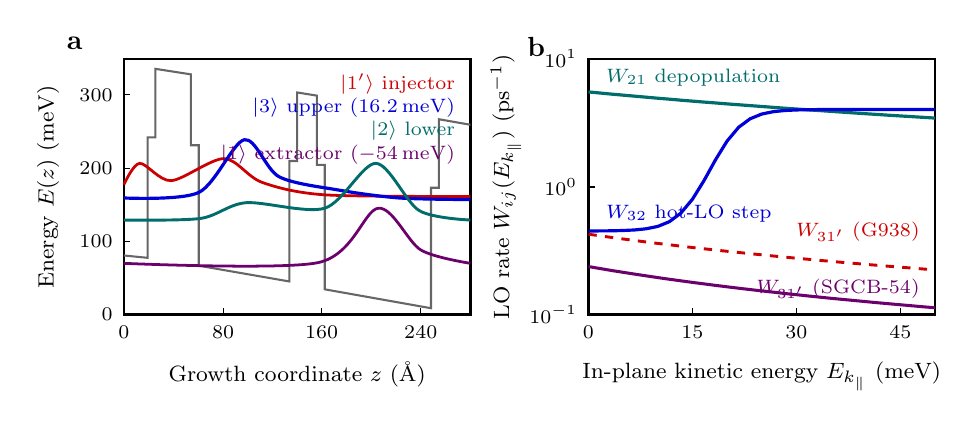
\begin{tikzpicture}[x=1cm,y=1cm,font=\footnotesize]
  % Panel a: Subband wavefunctions of SGCB-54 at F = 30.2 kV/cm
  \node[anchor=north west,font=\bfseries\normalsize] at (0.10,4.35) {a};
  \draw[thick] (0.95,0.70) rectangle (5.35,3.95);
  \foreach \v/\y in {0/0.70, 100/1.63, 200/2.56, 300/3.49} {
    \draw (0.95,\y) -- (1.03,\y);
    \node[left,font=\scriptsize] at (0.93,\y) {\v};
  }
  \foreach \xval/\xpos in {0/0.95, 80/2.21, 160/3.46, 240/4.72} {
    \draw (\xpos,0.70) -- (\xpos,0.78);
    \node[below,font=\scriptsize] at (\xpos,0.68) {\xval};
  }
  \node[below,font=\footnotesize] at (3.15,0.22) {Growth coordinate $z$ (\AA)};
  \node[rotate=90,above,font=\footnotesize] at (0.25,2.32) {Energy $E(z)$ (meV)};

  % Tilted conduction band profile with step-graded barriers
  \draw[black!60,line width=0.75pt]
    (0.95,1.45) -- (1.25,1.42) -- (1.25,2.95) -- (1.35,2.95) -- (1.35,3.82) -- (1.80,3.75) -- (1.80,2.85) -- (1.90,2.85)
    -- (1.90,1.32) -- (3.05,1.12) -- (3.05,2.65) -- (3.15,2.65) -- (3.15,3.52) -- (3.40,3.48) -- (3.40,2.60) -- (3.50,2.60)
    -- (3.50,1.02) -- (4.85,0.78) -- (4.85,2.31) -- (4.95,2.31) -- (4.95,3.18) -- (5.35,3.11);

  \draw[red!80!black,line width=1.0pt,smooth]
    plot coordinates {(0.95,2.35) (1.15,2.62) (1.55,2.40) (2.22,2.68) (2.70,2.38) (3.50,2.22) (5.35,2.20)};
  \draw[blue!85!black,line width=1.15pt,smooth]
    plot coordinates {(0.95,2.18) (1.90,2.25) (2.48,2.92) (2.92,2.45) (3.68,2.28) (4.45,2.18) (5.35,2.16)};
  \draw[teal!85!black,line width=1.05pt,smooth]
    plot coordinates {(0.95,1.90) (1.92,1.92) (2.50,2.12) (3.50,2.05) (4.15,2.62) (4.70,2.02) (5.35,1.90)};
  \draw[violet!85!black,line width=1.0pt,smooth]
    plot coordinates {(0.95,1.35) (3.42,1.36) (4.18,2.05) (4.72,1.52) (5.35,1.35)};

  \node[anchor=north east,font=\scriptsize,red!80!black] at (5.28,3.88) {$|1'\rangle$ injector};
  \node[anchor=north east,font=\scriptsize,blue!85!black] at (5.28,3.58) {$|3\rangle$ upper ($16.2\,\mathrm{meV}$)};
  \node[anchor=north east,font=\scriptsize,teal!85!black] at (5.28,3.28) {$|2\rangle$ lower};
  \node[anchor=north east,font=\scriptsize,violet!85!black] at (5.28,2.98) {$|1\rangle$ extractor ($-54\,\mathrm{meV}$)};

  % Panel b: k_parallel resolved LO phonon rates
  \node[anchor=north west,font=\bfseries\normalsize] at (5.95,4.35) {b};
  \draw[thick] (6.85,0.70) rectangle (11.25,3.95);
  \foreach \lbl/\y in {$10^{-1}$/0.70, $10^{0}$/2.32, $10^{1}$/3.95} {
    \draw (6.85,\y) -- (6.93,\y);
    \node[left,font=\scriptsize] at (6.83,\y) {\lbl};
  }
  \foreach \xval/\xpos in {0/6.85, 15/8.17, 30/9.49, 45/10.81} {
    \draw (\xpos,0.70) -- (\xpos,0.78);
    \node[below,font=\scriptsize] at (\xpos,0.68) {\xval};
  }
  \node[below,font=\footnotesize] at (9.05,0.22) {In-plane kinetic energy $E_{k_\parallel}$ (meV)};
  \node[rotate=90,above,font=\footnotesize] at (6.12,2.32) {LO rate $W_{ij}(E_{k_\parallel})$ ($\mathrm{ps}^{-1}$)};

  \draw[teal!85!black,line width=1.15pt] (6.850,3.527) -- (6.997,3.513) -- (7.143,3.499) -- (7.290,3.486) -- (7.437,3.473) -- (7.583,3.460) -- (7.730,3.447) -- (7.877,3.435) -- (8.023,3.422) -- (8.170,3.410) -- (8.317,3.398) -- (8.463,3.387) -- (8.610,3.375) -- (8.757,3.364) -- (8.903,3.353) -- (9.050,3.342) -- (9.197,3.331) -- (9.343,3.320) -- (9.490,3.310) -- (9.637,3.300) -- (9.783,3.290) -- (9.930,3.280) -- (10.077,3.270) -- (10.223,3.260) -- (10.370,3.250) -- (10.517,3.241) -- (10.663,3.231) -- (10.810,3.222) -- (10.957,3.213) -- (11.103,3.204) -- (11.250,3.195);
  \draw[blue!85!black,line width=1.15pt] (6.850,1.761) -- (6.997,1.762) -- (7.143,1.763) -- (7.290,1.767) -- (7.437,1.774) -- (7.583,1.789) -- (7.730,1.819) -- (7.877,1.879) -- (8.023,1.988) -- (8.170,2.164) -- (8.317,2.401) -- (8.463,2.665) -- (8.610,2.903) -- (8.757,3.078) -- (8.903,3.186) -- (9.050,3.246) -- (9.197,3.276) -- (9.343,3.291) -- (9.490,3.298) -- (9.637,3.301) -- (9.783,3.303) -- (9.930,3.304) -- (10.077,3.304) -- (10.223,3.304) -- (10.370,3.304) -- (10.517,3.304) -- (10.663,3.304) -- (10.810,3.304) -- (10.957,3.304) -- (11.103,3.304) -- (11.250,3.304);
  \draw[red!80!black,dashed,line width=1.05pt] (6.850,1.720) -- (6.997,1.699) -- (7.143,1.679) -- (7.290,1.659) -- (7.437,1.640) -- (7.583,1.621) -- (7.730,1.603) -- (7.877,1.586) -- (8.023,1.568) -- (8.170,1.551) -- (8.317,1.535) -- (8.463,1.519) -- (8.610,1.503) -- (8.757,1.488) -- (8.903,1.473) -- (9.050,1.458) -- (9.197,1.443) -- (9.343,1.429) -- (9.490,1.415) -- (9.637,1.402) -- (9.783,1.388) -- (9.930,1.375) -- (10.077,1.362) -- (10.223,1.350) -- (10.370,1.337) -- (10.517,1.325) -- (10.663,1.313) -- (10.810,1.301) -- (10.957,1.290) -- (11.103,1.278) -- (11.250,1.267);
  \draw[violet!85!black,line width=1.1pt] (6.850,1.309) -- (6.997,1.284) -- (7.143,1.259) -- (7.290,1.236) -- (7.437,1.213) -- (7.583,1.191) -- (7.730,1.169) -- (7.877,1.148) -- (8.023,1.128) -- (8.170,1.108) -- (8.317,1.089) -- (8.463,1.070) -- (8.610,1.052) -- (8.757,1.034) -- (8.903,1.017) -- (9.050,1.000) -- (9.197,0.984) -- (9.343,0.967) -- (9.490,0.952) -- (9.637,0.936) -- (9.783,0.921) -- (9.930,0.906) -- (10.077,0.892) -- (10.223,0.878) -- (10.370,0.864) -- (10.517,0.850) -- (10.663,0.837) -- (10.810,0.824) -- (10.957,0.811) -- (11.103,0.798) -- (11.250,0.786);

  \node[anchor=south west,font=\scriptsize,teal!85!black] at (6.95,3.48) {$W_{21}$ depopulation};
  \node[anchor=north west,font=\scriptsize,blue!85!black] at (6.95,2.22) {$W_{32}$ hot-LO step};
  \node[anchor=south east,font=\scriptsize,red!80!black] at (11.18,1.50) {$W_{31'}$ (G938)};
  \node[anchor=south east,font=\scriptsize,violet!85!black] at (11.18,0.78) {$W_{31'}$ (SGCB-54)};
\end{tikzpicture}
